\thispagestyle{headfootimage}

\titleformat{\subsection}
{\Large\bfseries\scshape\raggedright}
{\thesubsection}{1em}
{}
\titleformat{\subsubsection}
{\Large\bfseries\scshape\raggedright}
{\thesubsubsection}{1em}
{}
\titlespacing*{\section}{0pt}{*.9}{*.9}
\titlespacing*{\subsection}{0pt}{*0.5}{*0}
\titlespacing*{\subsubsection}{1cm}{*0}{*0}

%\newenvironment{subapend}{\begin{adjustwidth}{0.1\textwidth}{0cm}}{\end{adjustwidth}}
%\newenvironment{subsubapend}{\begin{adjustwidth}{0.1\textwidth}{0cm}}{\end{adjustwidth}}

\chapter{}
Este apêndice apresenta os gráficos referentes a geração pontual em cada mês entre os anos de 2014 e 2017. Nele pode-se perceber que os momentos onde ocorrem maior geração anual acontecem nos meses de janeiro, novembro e dezembro para a maioria dos dias de coleta. Essa tendência pode ser percebida principalmente para as segundas-feira, quando os pontos ultrapassam a média de geração para as segundas-feiras. Para quarta e sexta-feira, os valores ultrapassam a média anual com maior frequência nos meses mencionados.

%\section{Segundas-feira}

\begin{landscape}
	
	\begin{figure}[h]
		\centering
		\caption*{Segundas-Feira}
		\begin{minipage}{1.3\textwidth}
			\centering
			\label{fig:image111}
			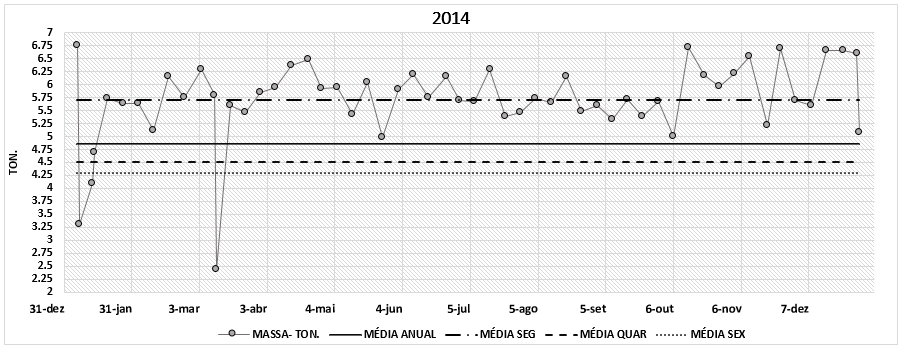
\includegraphics[width=1\textwidth]{produtos/prodtres/image111}
		\end{minipage}
		\begin{minipage}{1.3\textwidth}
			\centering
			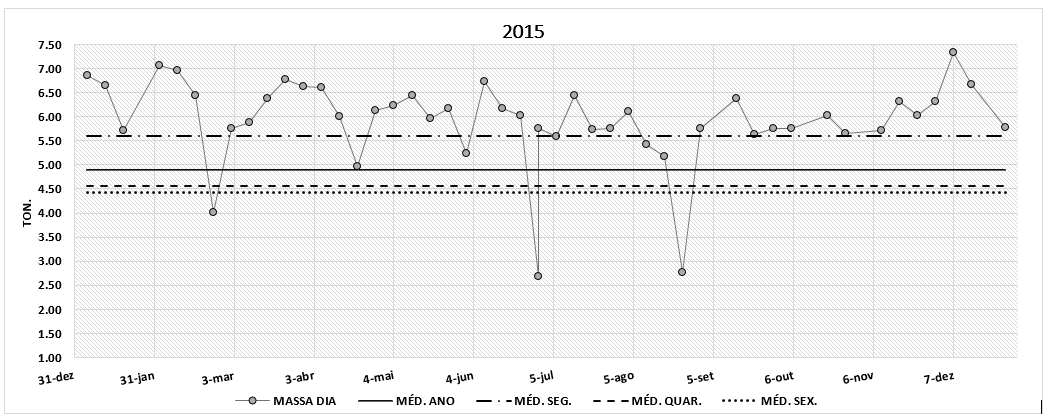
\includegraphics[width=1\textwidth]{produtos/prodtres/image112}
			\label{fig:image112}
		\end{minipage}
	\end{figure}
	
		\begin{figure}[h]
		\centering
		\caption*{Segundas-feira}
		\begin{minipage}{1.4\textwidth}
			\centering
			\label{fig:image113}
			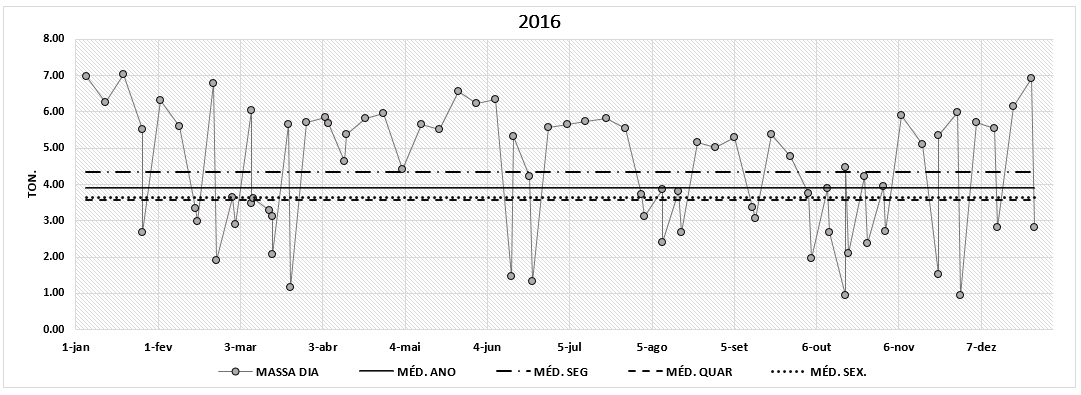
\includegraphics[width=1\textwidth]{produtos/prodtres/image113}
		\end{minipage}
		\begin{minipage}{1.4\textwidth}
			\centering
			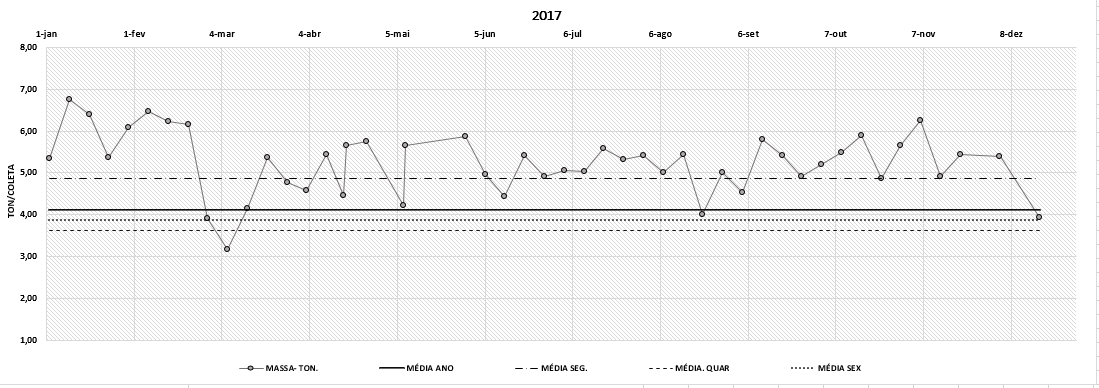
\includegraphics[width=1\textwidth]{produtos/prodtres/image114}
			\label{fig:image114}
		\end{minipage}
	\end{figure}

\end{landscape}

\FloatBarrier

%\section{Quartas-feira}

\begin{landscape}
	
	\begin{figure}[h]
		\centering
		\caption*{Quartas-feira}
		\begin{minipage}{1.4\textwidth}
			\centering
			\label{fig:image115}
			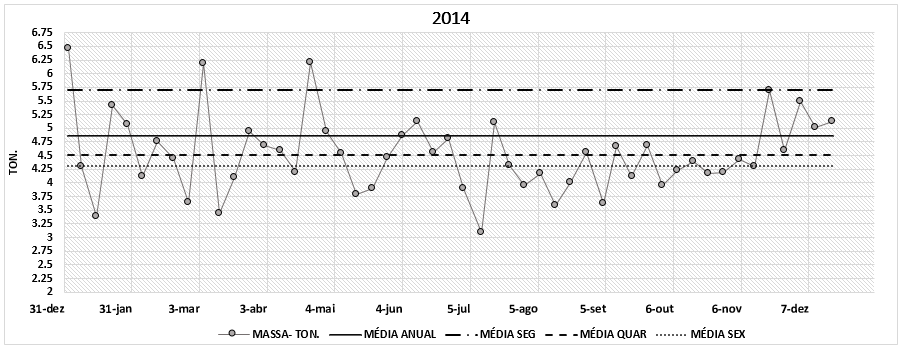
\includegraphics[width=1\textwidth]{produtos/prodtres/image115}
		\end{minipage}
		\begin{minipage}{1.4\textwidth}
			\centering
			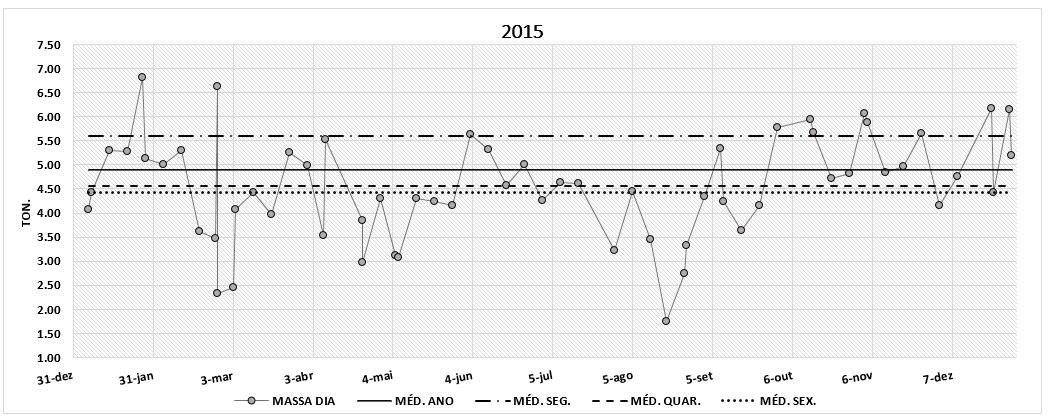
\includegraphics[width=1\textwidth]{produtos/prodtres/image116}
			\label{fig:image116}
		\end{minipage}
	\end{figure}
	
	\begin{figure}[h]
		\centering
		\caption*{Quartas-feira}
		\begin{minipage}{1.4\textwidth}
			\centering
			\label{fig:image118}
			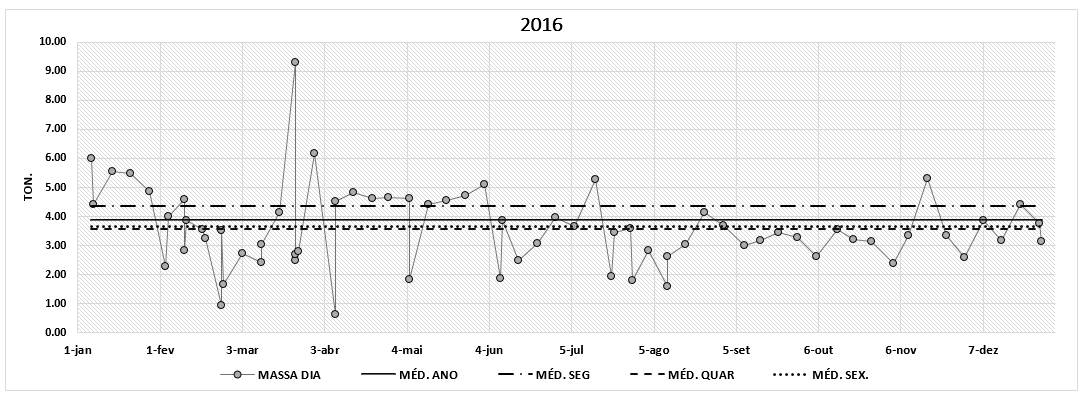
\includegraphics[width=1\textwidth]{produtos/prodtres/image118}
		\end{minipage}
		\begin{minipage}{1.4\textwidth}
			\centering
			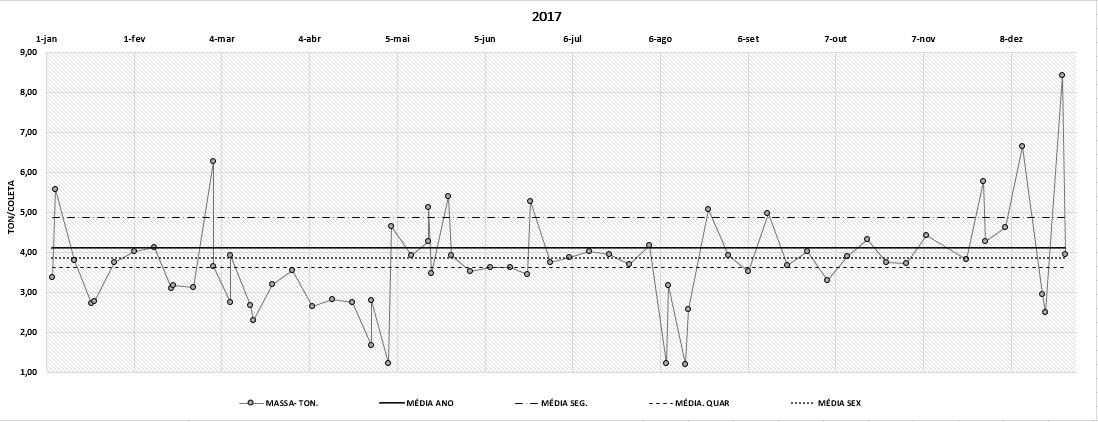
\includegraphics[width=1\textwidth]{produtos/prodtres/image117}
			\label{fig:image117}
		\end{minipage}
	\end{figure}
	
\end{landscape}

\FloatBarrier

%\section{Sextas-feira}

\begin{landscape}
	
	\begin{figure}[h]
		\centering
		\caption*{Sextas-feira}
		\begin{minipage}{1.4\textwidth}
			\centering
			\label{fig:image119}
			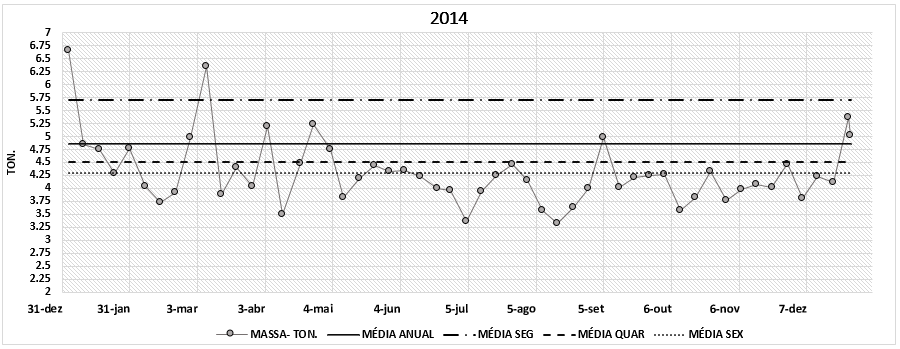
\includegraphics[width=1\textwidth]{produtos/prodtres/image119}
		\end{minipage}
		\begin{minipage}{1.4\textwidth}
			\centering
			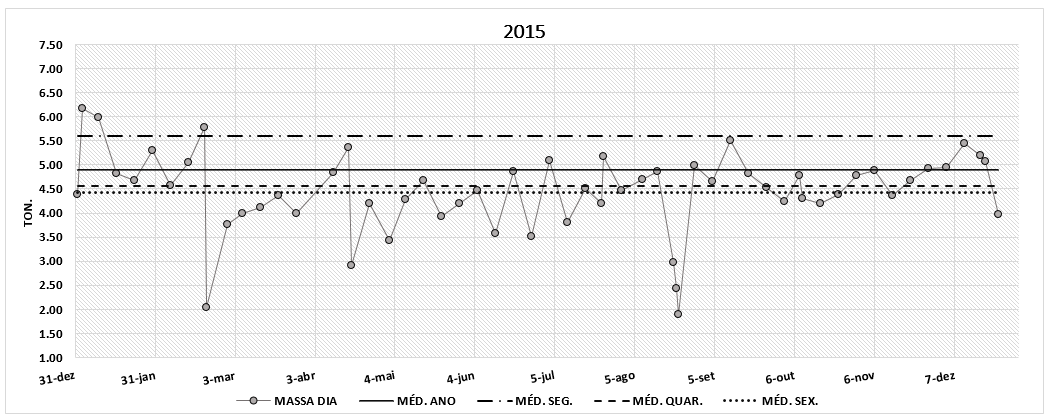
\includegraphics[width=1\textwidth]{produtos/prodtres/image120}
			\label{fig:image120}
		\end{minipage}
	\end{figure}
	
	\begin{figure}[h]
		\centering
		\caption*{Sextas-feira}
		\begin{minipage}{1.4\textwidth}
			\centering
			\label{fig:image121}
			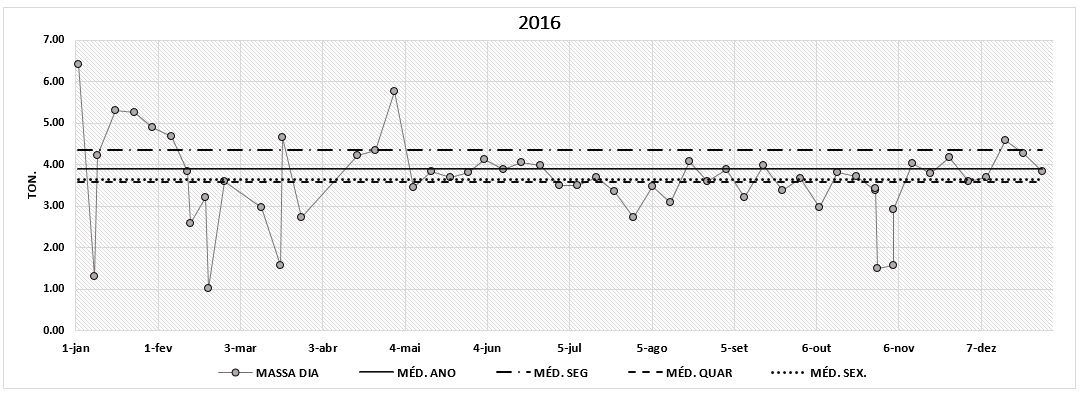
\includegraphics[width=1\textwidth]{produtos/prodtres/image121}
		\end{minipage}
		\begin{minipage}{1.4\textwidth}
			\centering
			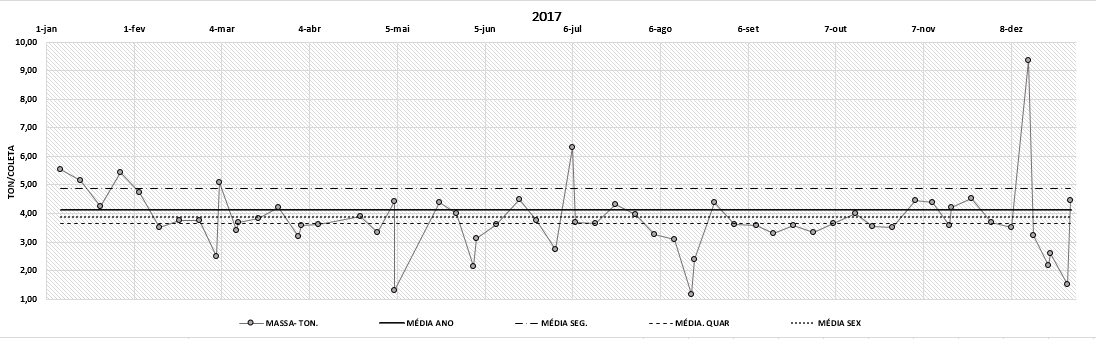
\includegraphics[width=1\textwidth]{produtos/prodtres/image122}
			\label{fig:image122}
		\end{minipage}
	\end{figure}
	
\end{landscape}

\FloatBarrier

\chapter{}

Este apêndice apresenta as Listas de Presença referentes as Oficinas Participativas realizadas no município de Monteiro Lobato, no período de agosto a outubro de 2018. A metodologia e resultados para essas Oficinas encontram-se descritas na secção \ref{oficinas} deste produto.

\newpage
\section{Oficina participativa com os professores}

\begin{figure}[h]
	\centering
	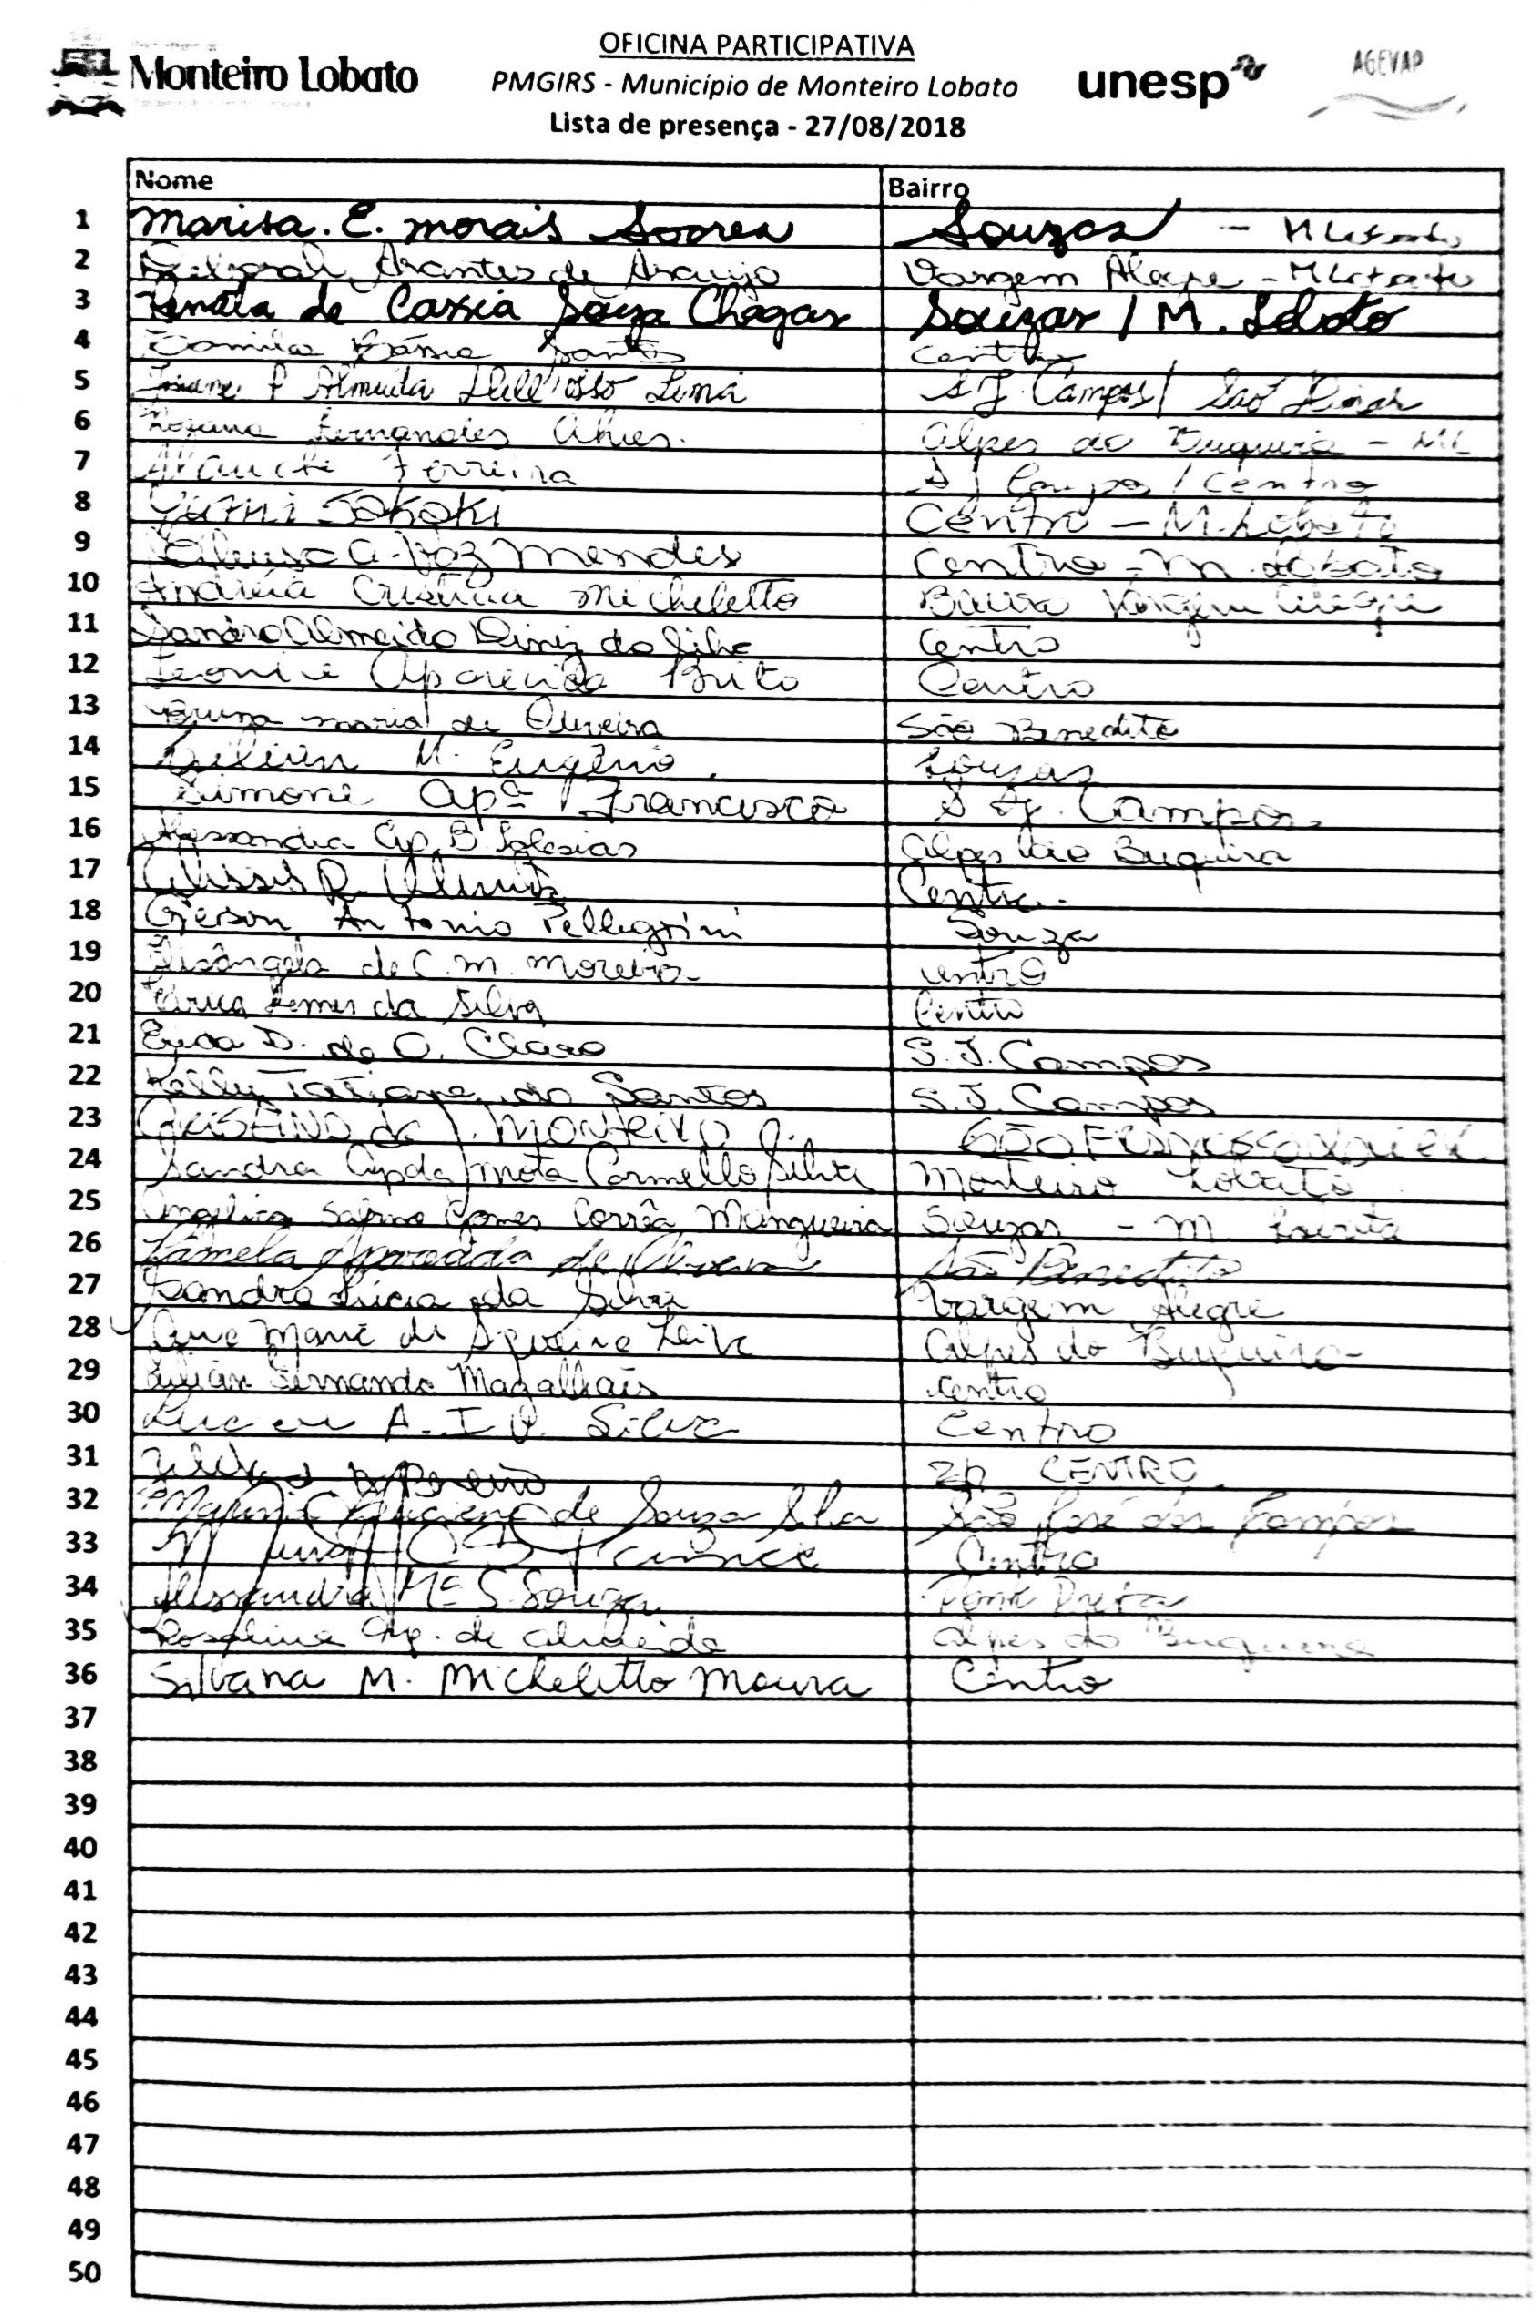
\includegraphics[width=.75\linewidth]{produtos/prodtres/image123}
	\caption*{}
	\label{fig:image123}
\end{figure}

\FloatBarrier
\newpage
\section{Oficina participativa com o bairro centro}
\begin{figure}[h]
	\centering
	
\includegraphics[width=.75\linewidth]{produtos/prodtres/image124}
	\caption*{}
	\label{fig:image124}
\end{figure}

\FloatBarrier
\newpage
\section{Oficina participativa com o bairro Souzas}
\begin{figure}[h]
	\centering
	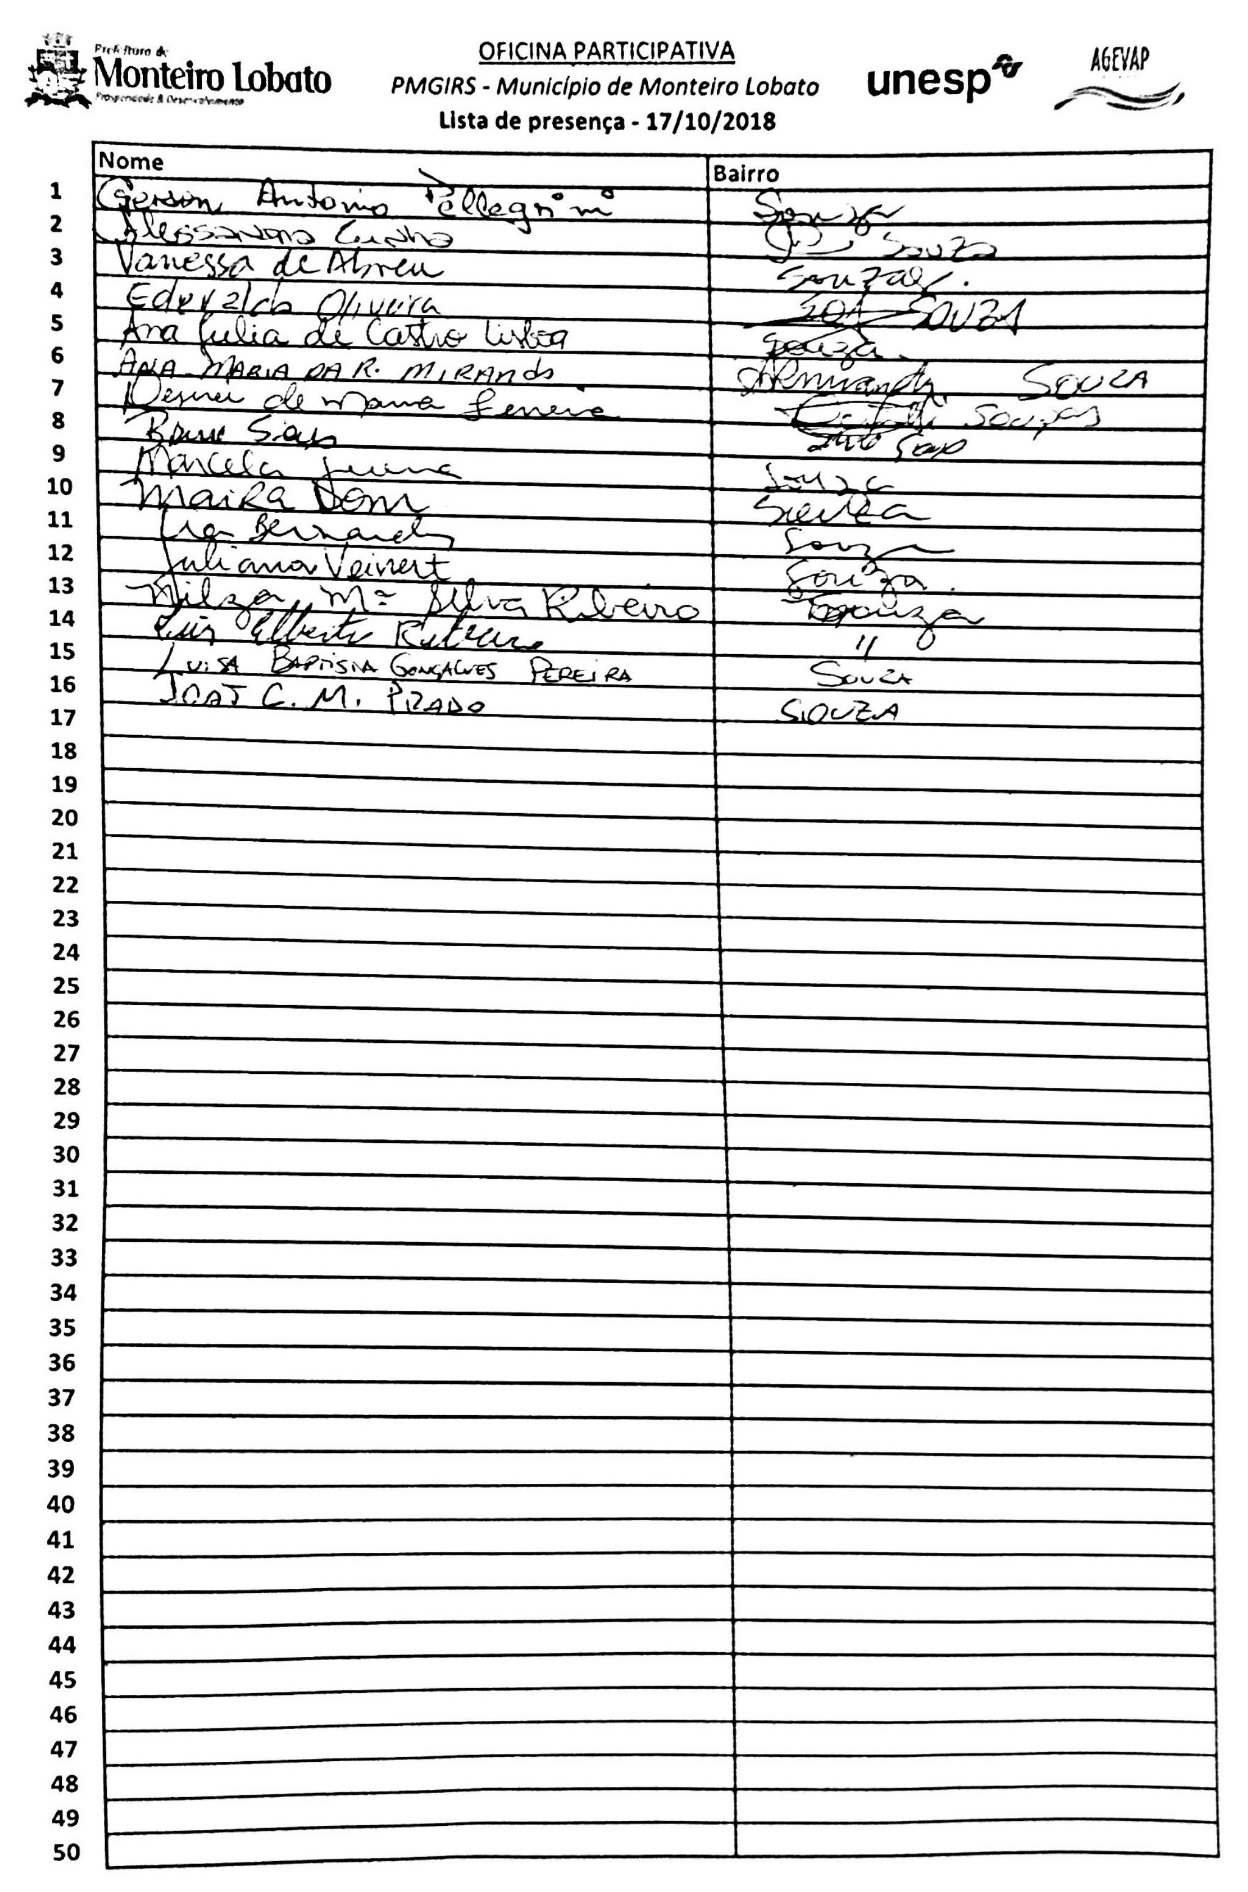
\includegraphics[width=.75\linewidth]{produtos/prodtres/image125}
	\caption*{}
	\label{fig:image125}
\end{figure}

\FloatBarrier
\newpage
\section{Oficina participativa com o bairro São Benedito}
\begin{figure}[h]
	\centering
	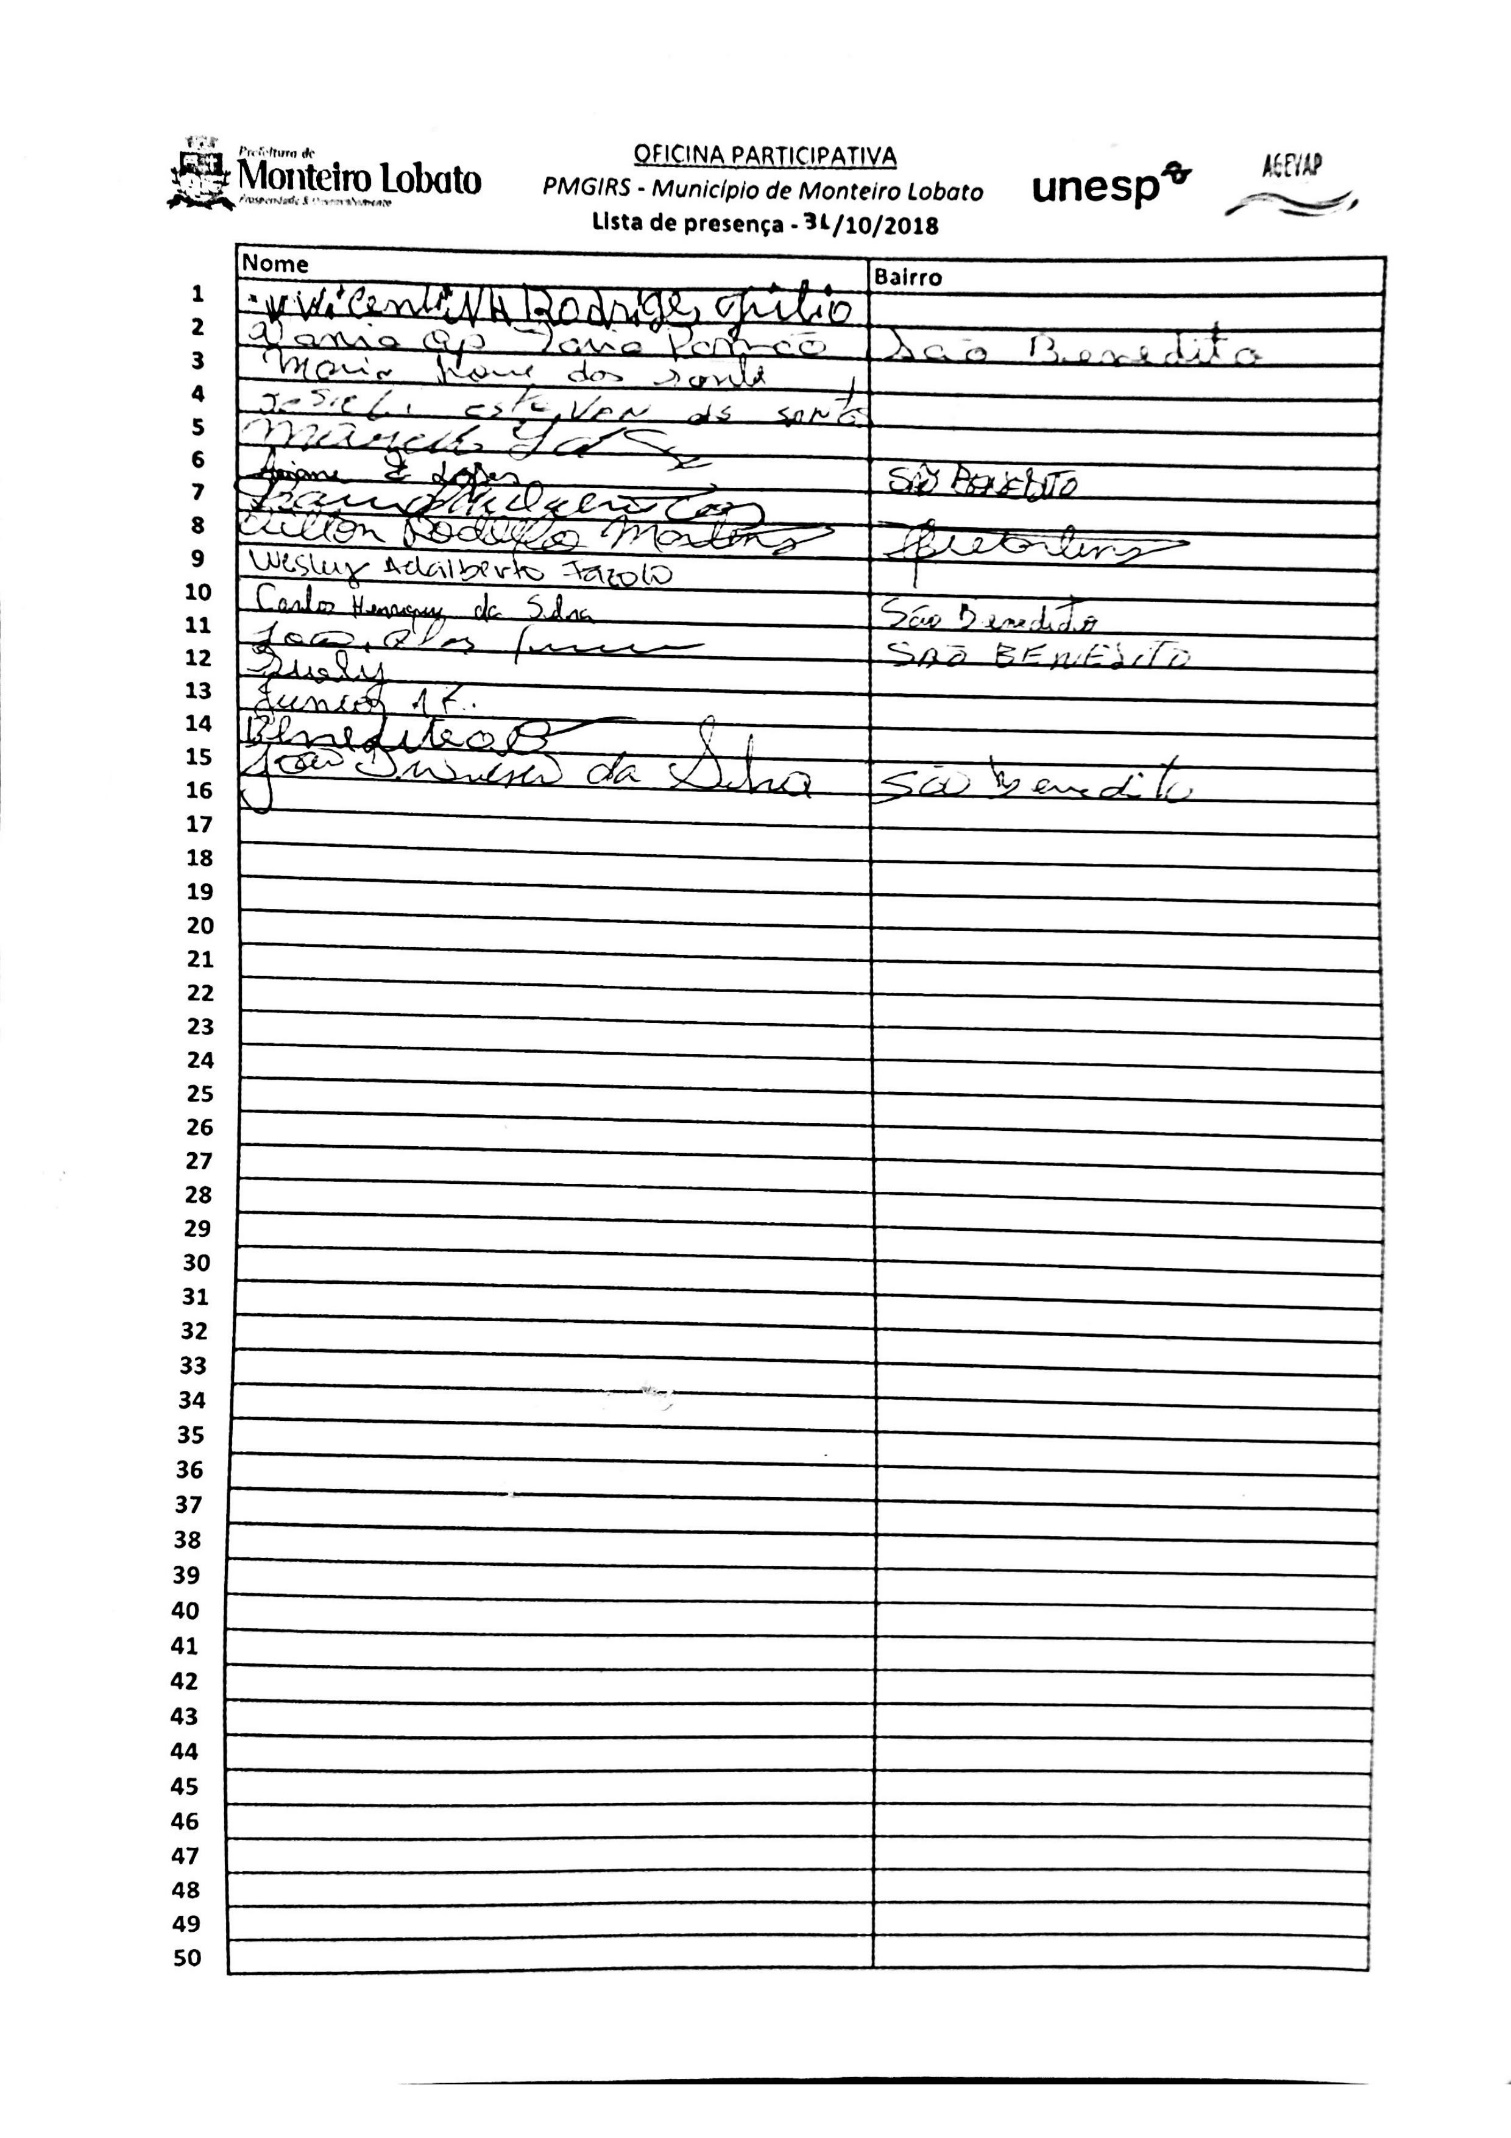
\includegraphics[width=.75\linewidth]{produtos/prodtres/image126}
	\caption*{}
	\label{fig:image126}
\end{figure}
